% Fully-connected MLP: layers of 3, 4, 4, 2 neurons.
% White-filled circles, mid-thick grey outline, thin grey connections.
\documentclass[tikz,border=4pt]{standalone}
\usepackage{tikz}
\usepackage{xcolor}
\usetikzlibrary{positioning, calc, arrows.meta}

\begin{document}
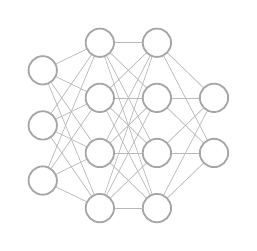
\begin{tikzpicture}[
  font=\sffamily\footnotesize,
]
% layer x positions (halved horizontal spacing)
\pgfmathsetmacro{\xA}{0.000}
\pgfmathsetmacro{\xB}{0.725}
\pgfmathsetmacro{\xC}{1.450}
\pgfmathsetmacro{\xD}{2.175}

% vertical step between neurons
\pgfmathsetmacro{\vs}{0.70}

% neuron radius
\pgfmathsetmacro{\nr}{0.18}

% ---- neuron coordinates (centered on y=0) ----
% layer A: 3 neurons -> y in {-1, 0, 1} * vs
\foreach \i [count=\k from 0] in {-1, 0, 1} {
  \coordinate (A\k) at (\xA, \i*\vs);
}
% layer B: 4 neurons -> y in {-1.5, -0.5, 0.5, 1.5} * vs
\foreach \i [count=\k from 0] in {-1.5, -0.5, 0.5, 1.5} {
  \coordinate (B\k) at (\xB, \i*\vs);
}
% layer C: 4 neurons
\foreach \i [count=\k from 0] in {-1.5, -0.5, 0.5, 1.5} {
  \coordinate (C\k) at (\xC, \i*\vs);
}
% layer D: 2 neurons -> y in {-0.5, 0.5} * vs
\foreach \i [count=\k from 0] in {-0.5, 0.5} {
  \coordinate (D\k) at (\xD, \i*\vs);
}

% ---- connection lines (drawn before circles so neurons sit on top) ----
\foreach \a in {0,1,2}{%
  \foreach \b in {0,1,2,3}{%
    \draw[gray!55, line width=0.25pt] (A\a) -- (B\b);
  }
}
\foreach \a in {0,1,2,3}{%
  \foreach \b in {0,1,2,3}{%
    \draw[gray!55, line width=0.25pt] (B\a) -- (C\b);
  }
}
\foreach \a in {0,1,2,3}{%
  \foreach \b in {0,1}{%
    \draw[gray!55, line width=0.25pt] (C\a) -- (D\b);
  }
}

% ---- neurons ----
\foreach \name in {A0,A1,A2, B0,B1,B2,B3, C0,C1,C2,C3, D0,D1}{
  \fill[white] (\name) circle (\nr);
  \draw[gray!70, line width=0.65pt] (\name) circle (\nr);
}

\end{tikzpicture}
\end{document}
